\documentclass[colorlinks]{article}
\usepackage{graphicx}

\usepackage{hyperref,verbatim}
\usepackage[usenames, dvipsnames]{color}
\usepackage{tgpagella} % text only
\usepackage{mathpazo} 
\usepackage[margin=0.6in]{geometry}
\addtolength{\topmargin}{0in}


\newcommand{\deadline}{Noon Jan 15}
\newcommand{\extdeadline}{Noon Jan 16}
\newcommand{\total}{18}

%opening
\title{Machine Learning\\Homework 1 : Decision Trees\\(due \deadline)}
\author{}
\date{}

\begin{document}

\maketitle

\noindent\fbox{
	\parbox{\textwidth}{
		Instructions\\
		\begin{enumerate}
			\item In case you are unfamiliar with the Python data ecosystem (NumPy, Pandas), you are recommended to study the first four chapters of the \href{https://jakevdp.github.io/PythonDataScienceHandbook/}{Python data science handbook}. A doubt clearing session would be organised in case you have any difficulties in the data science ecosystem.
			\item The deadline for full score is \deadline. You can get 50\% credit for late submission (\extdeadline).
			\item Total marks = \total
			\item You have to type the assignment using a word processing engine, create a pdf and upload on the form. Please note that only pdf files will be accepted.
			\item All code/Jupyter notebooks must be put up as \href{https://gist.github.com/}{\textbf{secret gists}} and linked in the created pdf submission. Again, only secret gists. Not public ones.
			\item Any instances of cheating/plagiarism will not be tolerated at all. 
			\item Cite all the pertinent references in IEEE format.
			\item The least count of grading would be 0.5 marks. 

		\end{enumerate}
	}
}

\begin{figure}
	\centering
	\vspace{-100pt}
	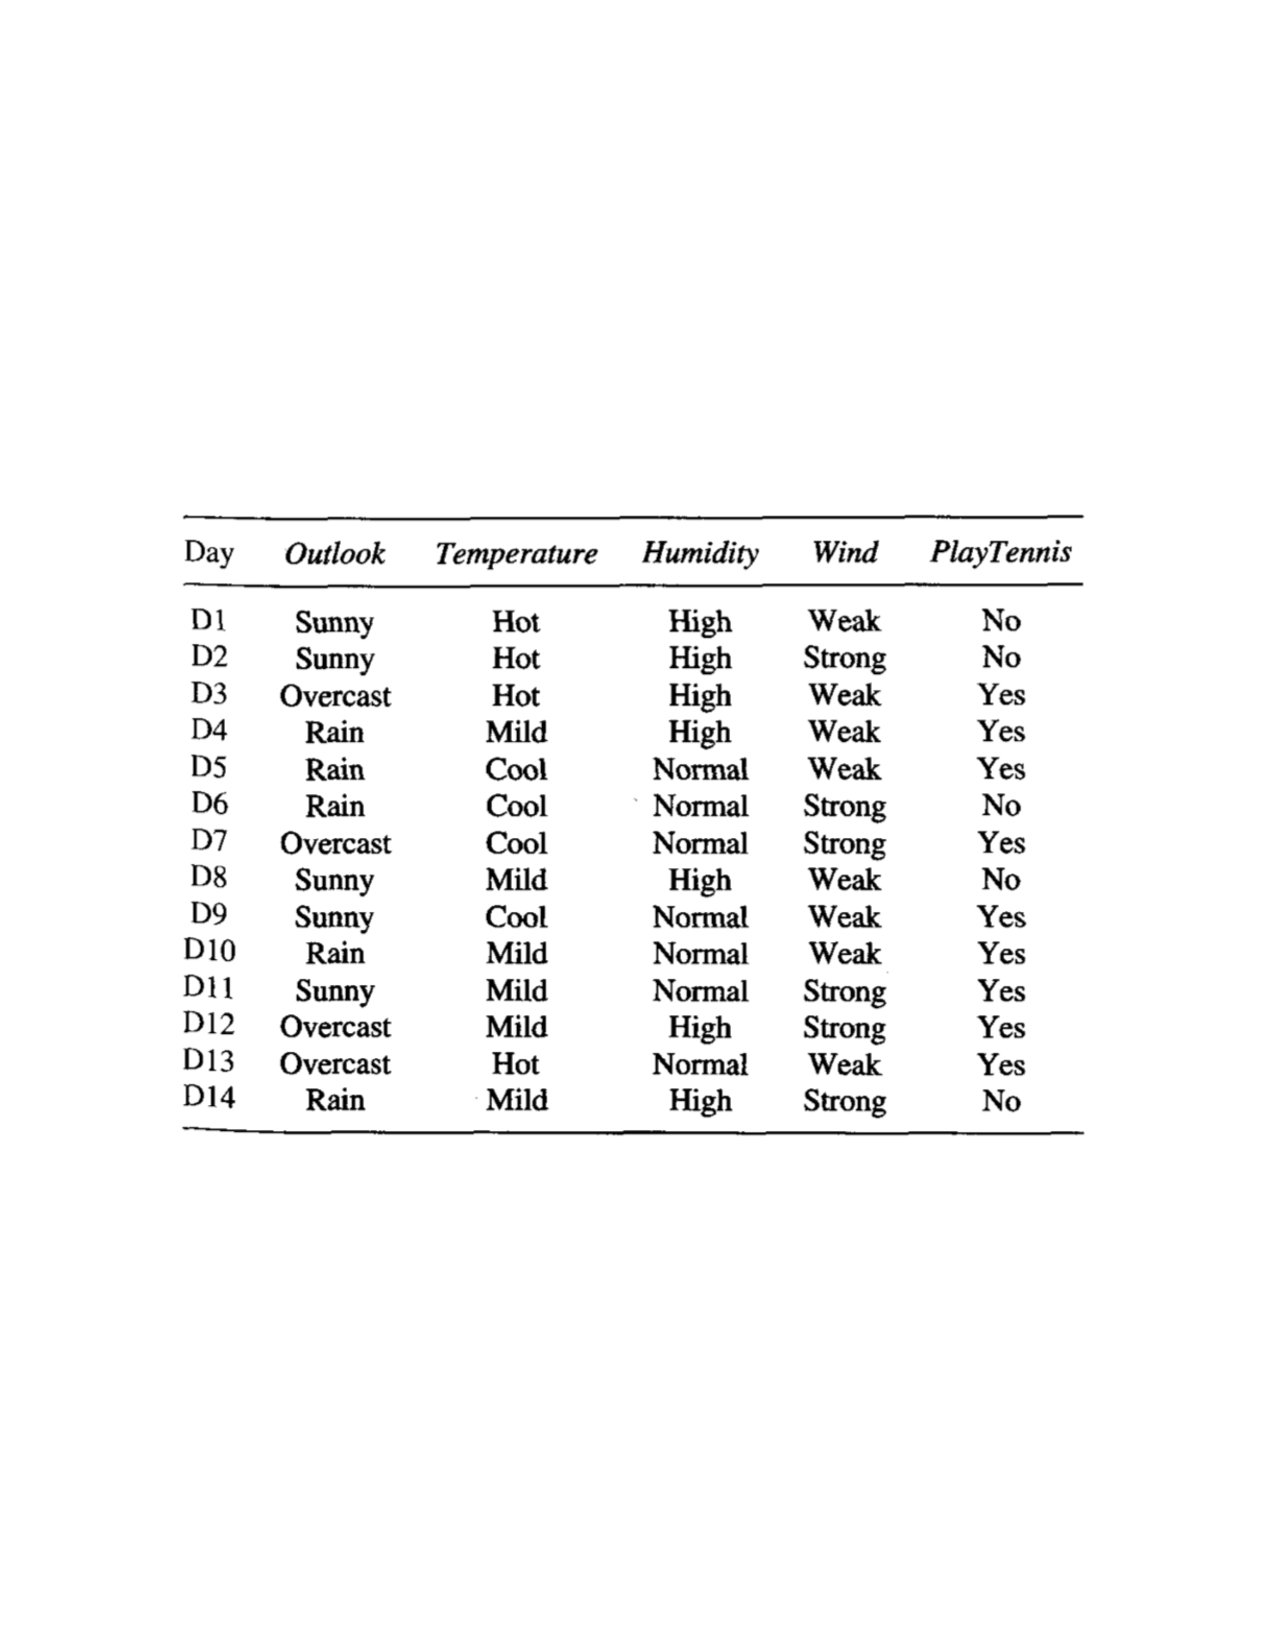
\includegraphics[scale=0.5]{dt-dataset.pdf}
	\vspace{-100pt}
	\caption{PlayTennis Dataset}
	\label{fig:dt-dataset}
\end{figure}




\begin{enumerate}
	\item Modify the code in the Github repository (as shared via Githu)
	\item 	\begin{enumerate}
		\item For the following dataset shown in Figure~\ref{fig:dt-dataset}(~same as the one we used in the class), now let us assume that date is also an input feature. Which attribute will be chosen as the root node for the decision tree? Do you think choosing this attribute is a good choice? Explain your answer.  \textbf{[1 mark]}
	\end{enumerate}



\item 	\begin{enumerate}
	

	
		\item Complete the decision tree implementation from scratch filling the code todos in the Github repository. The code should be written in native Python and not use existing libraries. The code should work for regression and classification tasks. As a hint: you may want to use dictionaries to encode the nested relationship amongst the different nodes, eg. tree = \`feature1' :\{`val1': ..., `val2', ...\}\}. \textbf{[4 marks]}
		\item Show the usage of your decision tree on the IRIS dataset. The first 70\% of the data should be used for training purposes and the remaining 30\% for test purposes. Show the accuracy of the decision tree you implemented on the test dataset. \textbf{[1 mark]}
		\item Also, write the code for the plotting function to create an ASCII display for the learnt decision tree \textbf{[1 mark]}
		\item Use 5 fold cross-validation on the dataset. Using nested cross-validation find the optimum depth of the tree. \textbf{[2 marks]}
	\end{enumerate} 
	
	\item Show the usage of your decision tree for the \href{https://archive.ics.uci.edu/ml/datasets/Real+estate+valuation+data+set}{real estate price prediction regression} problem. \textbf{[1 mark]}
	\item Compare the performance of your model with the decision tree module from scikit learn. \textbf{[1 mark]}
	\item Create some fake data to do some experiments on the runtime complexity of your decision tree algorithm. Create a dataset with N samples and M binary features. Vary M and N to plot the time taken for: 1) learning the tree, 2) predicting for test data. How do these results compare with theoretical time complexity for decision tree creation and prediction. You should do the comparison for all the four cases of decision trees. \textbf{[2 marks]}	
	

\end{enumerate}


Some useful references for the homework:

\begin{enumerate}
	\item \href{https://scikit-learn.org/stable/modules/tree.html}{Scikit-learn page on decision trees}
		\item \href{https://scikit-learn.org/stable/modules/ensemble.html}{Scikit-learn page on ensemble methods}
\end{enumerate}







\end{document}
